%PSoC API modultest

PSoC APIen testet i PSoC creator med den indbyggede debug-funktion. I main filen skrives et lille test program som kan ses på figur \ref{lab:sht_testmain}.

\begin{figure}[htb]
\centering
{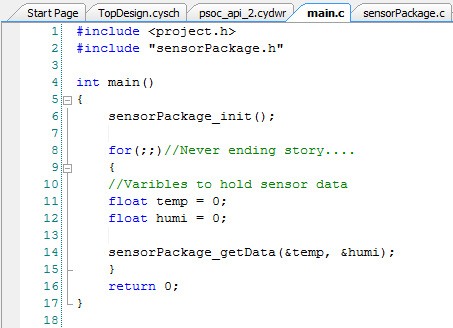
\includegraphics[width=0.70\textwidth]{filer/modultest/Billeder/psoc_testmain.png}}
\caption{main test program}
\label{lab:sht_testmain}
\end{figure}

Først initialiseres de nødvendige 'objekter' hvor opsætninger af komponenter også initialiseres. I en uendelig for-løkke oprettes to variabler til lagring af temperatur- og fugtighedsdata og disse sættes lige med nul. Derefter kaldes funktionen til aflæsning af data, denne kalder to funktioner, en for temperatur og en for fugtighed. Disse funktioner sørger selv for at sensorens select-ben bliver sat lav for temperatur og høj for fugtighed. 

ADCen forbindes til GND og VCC for at teste nogle værdier, dette vil give hvad der svarer til 0 og 100 \% duty cycle. 
  
\begin{figure}[htb]
\centering
{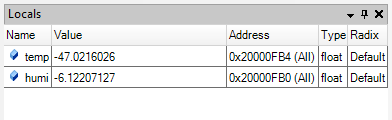
\includegraphics[width=0.70\textwidth]{filer/modultest/Billeder/psoc_api_test1.png}}
\caption{Resultat for ADC forbundet til GND}
\label{lab:sht_api_test1}
\end{figure}

\begin{figure}[htb]
\centering
{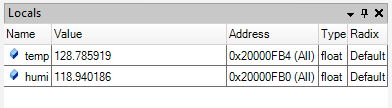
\includegraphics[width=0.70\textwidth]{filer/modultest/Billeder/psoc_api_test2.png}}
\caption{Resultat for ADC forbundet til VCC}
\label{lab:sht_api_test2}
\end{figure}

Under debug kan måleresultaterne aflæses som det ses på figur \ref{lab:sht_api_test1} og \ref{lab:sht_api_test2}. 
For 0 \% duty cycle vil $temp = -46,85$ og $fugt = -6,0$ i forhold til databladet.
for 100 \% duty cycle vil $temp = 128,9$ og $fugt = 119$ i forhold til databladet.
Fugtigheden er, som nævnt under design, kun defineret ved 0...100 \% duty cycle og ovenstående værdi er udelukkende teoretisk og bruges kun for at teste funktionen. 

Disse værdier stemmer godt overens, dog med en minimal afvigelse, med de udlæste værdier for debug og testen kan derfor antages som godkendt.